\section{Overview and Motivation (Implementation)}\label{sec:c6s1}
\lipsum[110-110]

This section builds on the material in \cref{ch:6}, \cref{ch:7} and the prior work of \citet{ch6-9}; see also \citep{ch6-12,ch6-11}.

\begin{align}\label{eq:c6s1-a}
  \mathbf{x}_{k+1} &= \mathbf{A}\mathbf{x}_k + \mathbf{B}\mathbf{u}_k + \mathbf{w}_k, & \mathbf{w}_k&\sim\mathcal{N}(0,\mathbf{Q}),\\
  \mathbf{y}_k &= \mathbf{C}\mathbf{x}_k + \mathbf{v}_k, & \mathbf{v}_k&\sim\mathcal{N}(0,\mathbf{R}).\label{eq:c6s1-b}
\end{align}

Equations~\eqref{eq:c6s1-a} and~\eqref{eq:c6s1-b} are used throughout the remainder of this section.

\kant[9-12]

\subsection{Quantitative behaviour}\label{sec:c6s1-q}
Results are collected in \cref{tab:c6s1} and visualised in \cref{fig:c6s1-f1}. Similar trends were reported in~\citep{ch6-10,ch6-3}.

\begin{table}[htbp]
\centering
\caption{Summary of measured quantities for experiment set \texttt{c6s1}.}\label{tab:c6s1}
\begin{tabular}{lrrr}
\toprule
Method & Score & Latency & Error \\
\midrule
Alpha & \num{77.4} & \SI{5.19}{\milli\second} & \num{8.036e-4} \\
Beta & \num{46.2} & \SI{2.32}{\milli\second} & \num{2.024e-1} \\
Gamma & \num{71.6} & \SI{1.90}{\milli\second} & \num{5.603e-5} \\
Delta & \num{86.7} & \SI{2.28}{\milli\second} & \num{5.243e-2} \\
Epsilon & \num{51.2} & \SI{6.19}{\milli\second} & \num{6.041e-1} \\
\bottomrule
\end{tabular}
\end{table}

\begin{figure}[htbp]
\centering
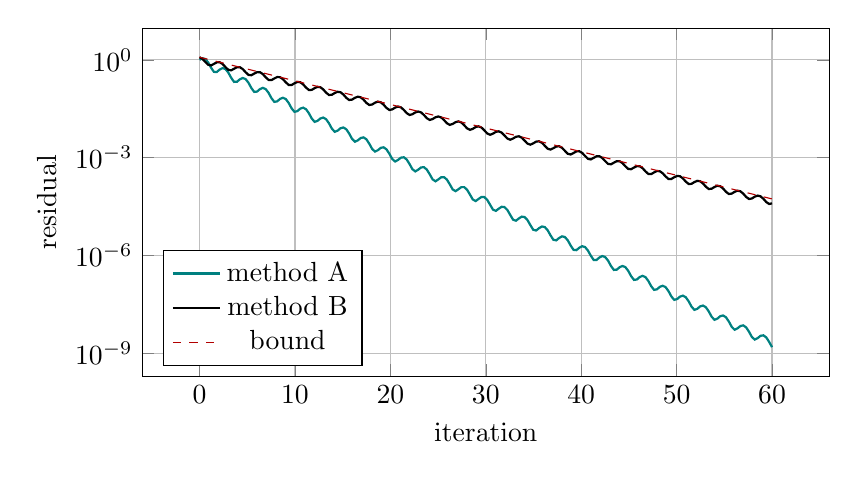
\begin{tikzpicture}\begin{semilogyaxis}[width=0.85\linewidth,height=6cm,xlabel={iteration},ylabel={residual},domain=0:60,grid=major,legend pos=south west]
\addplot[teal,thick,samples=200]{exp(-x/3)*(1+0.3*sin(deg(x*3)))};
\addplot[black,thick,samples=200]{exp(-x/6)*(1+0.2*cos(deg(x*3)))};
\addplot[red!70!black,dashed,samples=200]{1.2*exp(-x/6)};
\legend{method A,method B,bound}
\end{semilogyaxis}\end{tikzpicture}
\caption{Generated figure for \texttt{c6s1-f1} (parameters $a=3$, $b=3$).}\label{fig:c6s1-f1}
\end{figure}

\kant[9-11]

\subsection{Implementation notes}\label{sec:c6s1-i}
The core routine is shown in \cref{lst:c6s1}; its complexity is $\mathcal{O}(N\log N)$ per iteration~\cite{ch6-7}.

\begin{lstlisting}[language=python,caption={Reference implementation for c6s1.},label={lst:c6s1}]
def conjugate_gradient(A, b, tol=1e-8, maxit=500):
    x = b * 0
    r = b - A @ x
    p = r.copy()
    for k in range(maxit):
        Ap = A @ p
        alpha = (r @ r) / (p @ Ap)
        x += alpha * p
        r_new = r - alpha * Ap
        if (r_new @ r_new) ** 0.5 < tol:
            break
        p = r_new + ((r_new @ r_new) / (r @ r)) * p
        r = r_new
    return x
\end{lstlisting}

\kant[3-10]
\begin{theorem}\label{thm:c6s1}
Let $A\in\mathbb{R}^{n\times n}$ be symmetric positive definite with condition number $\kappa$. Then the iteration converges and
$\lVert e_k\rVert_A \le 2\bigl(\tfrac{\sqrt\kappa-1}{\sqrt\kappa+1}\bigr)^k\lVert e_0\rVert_A$.
\end{theorem}
\begin{enumerate}[label=(\roman*)]
\item the bound in \cref{thm:c6s1} is sharp for some initial errors;
\item the constant $2$ cannot be improved in general;
\item preconditioning reduces the effective $\kappa$.
\end{enumerate}

\lipsum[94-94]
